\section{Architectural Description}

\subsection{Overview}
	The logical structure of the service is divided in the following manner:
	\begin{description}
		\item[Client Interface Layer:] Its purpose is to interact with all types of users. This includes both a web interface, reserved for customers, and a mobile application,
			used by both customers and drivers.
		\item[Business and Web Layer:] This layer is responsible for the connection of the first layer with the Database Management Layer. It connects users to the information management
			system on the server. This layer operates server-side along with the Data Management Layer. It is also responsible for the management of driver queues and
			the creation of shared ride orders.
		\item[Database Management Layer:] This layer is responsible for both user information management as well as reservation storage. Other than saving important and sensitive
			information about the user, it also stores information about the reservations made by users. It communicates with the Business Layer on a event basis when shared rides
			are to be created or locked.
	\end{description}
\subsection{High Level Components and Their Interaction}

	\begin{figure}[h!]
		\centering
		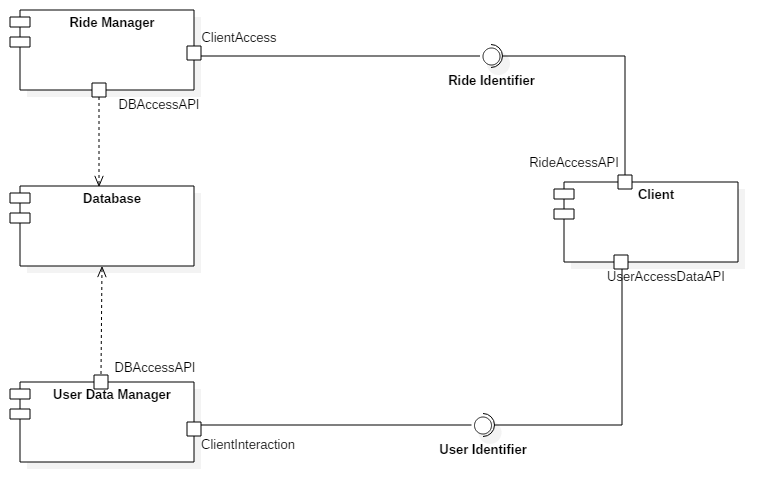
\includegraphics[width=0.9\textwidth]{components/Overview}
	\end{figure}

\subsection{Component View}
	\subsubsection{Client}
		\begin{figure}[h!]
			\centering
			\includegraphics[width=0.9\textwidth]{"components/Client View"}
		\end{figure}
	\subsubsection{Ride Manager}
		\begin{figure}[h!]
			\centering
			\includegraphics[width=0.9\textwidth]{"components/Ride Manager View"}
		\end{figure}

	\subsubsection{Data Manager}
		\begin{figure}[h!]
			\centering
			\includegraphics[width=0.9\textwidth]{"components/User Data Manager View"}
		\end{figure}



\subsection{Deployment View}
	\begin{figure}[h!]
			\centering
			\includegraphics[width=0.9\textwidth]{"components/DeploymentDiagram"}
	\end{figure}

\newpage

\subsection{Runtime View}
	\subsubsection{Sequence Diagram}
	In this section we show some service provided by our system to better understand how they work.
			\paragraph{Log In}
			In order to Log In the guest must: \begin{itemize}
				\item Open the service.
				\item Fill the fields with is account data.
			\end{itemize}
			During the Log In the system must check that:\begin{itemize}
				\item All the field are filled with valid data $($The first field must be an email and the second must follow the password rules$)$.
				\item The email is stored in the database and connected to an account.
				\item The emails-passwords must coincide.
			\end{itemize}
			\newpage
			\begin{figure}[h!]
				\centering
				\includegraphics[width=0.85\textwidth]{"SequenceDiagram/LogIn"}
			\end{figure}
			\newpage

		\paragraph{Instant Call}
			Both the guest and the user must tell their location to call a taxi.\\
			The system must:\begin{itemize}
				\item Check the location given by the guest/user.
				\item Extract from the queue the closest taxi to the given location.
				\item Send the request to the taxi driver.
				\item Confirm the request to the guest/user.
			\end{itemize}
			\begin{figure}[h!]
				\centering
				\includegraphics[width=0.85\textwidth]{"SequenceDiagram/InstantCall"}
			\end{figure}
			\newpage

		\paragraph{Taxi Reservation}
			A user can book a taxi with or without the sharing option by:\begin{itemize}
				\item Acces the booking {section}.
				\item Fill the requested fields.
			\end{itemize}
			The system must:\begin{itemize}
				\item Check the input given by the user.
				\item Update the Database.
			\end{itemize}
			\newpage
			\begin{figure}[h!]
				\centering
				\includegraphics[width=0.85\textwidth]{"SequenceDiagram/TaxiReservation"}
			\end{figure}
			\newpage

		\paragraph{Edit Boking}
			A user can edit a reservation by:\begin{itemize}
				\item Selecting the ride to edit from a list.
				\item Edit/cancels the ride.
			\end{itemize}
			The system must:\begin{itemize}
				\item Show the user's Booked Ride.
				\item Check if the ride can be edited.
				\item Check the new input given.
				\item Update the Database.
			\end{itemize}
				\newpage
				\begin{figure}[h!]
					\centering
					\includegraphics[width=0.85\textwidth]{"SequenceDiagram/EditBooked"}
				\end{figure}
				\newpage

			\paragraph{Accept/Refuse Call}
				The taxi driver must respond to a request sent by the system, and must notify the end of the ride.\\
				The system must:\begin{itemize}
					\item Push a notification to the first driver in the queue near the location of the ride.
					\item Check the answer.
					\item Handle the queue due to the answer given.
					\item Update the Database.
				\end{itemize}
				The Ride Manager gets a notification from a Database Trigger when a Ride is Locked .
				A notification is pushed instantly if it is an Instant Call or only a small time before the departure time of a Booked Ride.
				\newpage
				\begin{figure}[h!]
					\centering
					\includegraphics[width=0.85\textwidth]{"SequenceDiagram/Accept"}
				\end{figure}
				\newpage


\subsection{Component Interfaces}
	\subsubsection{Intra-component}
		\begin{description}
			\item[Ride Identifier]
				Methods contained within this interface are used to send data form the Client to the Ride Manager, to enable ride creation, modification and deletion. It is used for both
				reservations and instant calls. Methods here also allow taxi drivers to interact with rides, by "effectively" modifying the status of the rides.
			\item[User Identifier]
				This interface handles User access to the system. It has methods for both authentication and insertion of user data. All methods in this interface use end-to-end encryption
				to protect sensitive user data.
		\end{description}
	\subsubsection{Client}
		\begin{description}
			\item[Driver Access]
				This interface is used to access driver-only functions which regard the status of rides. It is used to retrieve ride information for the driver and allows a driver to set their working
				status and accept/refuse jobs.
			\item[User Access]
				This interface is used for authentication and access to the user information database.
			\item[Customer Request]
				This interface gives users the methods to do all things related to rides.
			\item[User ID]
				This interface gives separate methods to taxi driver users and regular customers to login to the service.
			\item[UI Access]
				Methods in this interface are used to render the graphical part of the mobile application.
		\end{description}
	\subsubsection{Ride Manager}
		\begin{description}
			\item[Ride Creation]
				This interface handles all incoming requests to edit and create rides.
			\item[Ride Accessor]
				This interface allows the creation and modification of ride objects inside the database. The modified objects have to be saved into the database afterwards.
			\item[Driver Management]
				This interface allow the controller to insert/remove a taxi driver into the queue and allows the controller to retrieve the first available driver in the queue to be assigned to
				a ride.
			\item[Data Modification]
				This interface is an intermediary between the controller and db accessor.
			\item[DBAccess]
				This interface handles database access.
		\end{description}
	\subsubsection{User Data Manager}
		\begin{description}
			\item[Data Editor]
				This interface takes all incoming requests to the data controller.
			\item[Authentication]
				The methods in this interface let users and drivers log in to the system.
			\item[User Data]
				This interface handles profile editing.
			\item[DBAccess]
				This interface deals with database access.
		\end{description}
\subsection{Selected Architectural Styles and Patterns}

\subsection{Further Design Choices}
